\section{3-D Macrophysics}

Despite the value of 1-D stellar evolution codes, stars are 3-D objects that exhibit non-spherical features.
The simplifications made by spherical symmetry and the MLT approximation do not sufficiently capture the 3-D physics of convection.
Because of this, there are modelling inconsistencies between 1-D MLT predictions and 3-D hydrodynamic simulations.

\subsection{Insufficiencies of MLT}

As explained before, MLT assumes that there is some average length $\ell_{\mathrm{MLT}}$ that all fluid elements travel in a convective environment before mixing with their surroundings.

One of the problems with MLT is how it treats the boundaries of a convective region where we find $\nabla_{\mathrm{ad}} = \nabla_{\mathrm{rad}}$.
According to Equation \ref{eq:d_mlt}, the diffusive coefficient for mixing is equal to the convective velocities.
Outside the boundary of a convective region, suddenly $v_{\mathrm{conv}} = 0$ which would imply an unphysical infinite acceleration to stop the fluid at the edges.
To more accurately treat the boundaries, stellar evolution codes like \texttt{MESA} implement a convective overshooting parameterization where 
\begin{equation}\label{eq:d_overshoot}
    D_{\mathrm{OV}} = D_{\mathrm{conv,0}}\times\exp{\Biggl(-\frac{2z}{f\lambda_{P,0}}\Biggr)}
\end{equation}
where $D_{\mathrm{conv,0}}$ is the diffusion coefficient at the boundary, $\lambda_{P,0}$ is the pressure scale height at that location, $z$ is the position in the radiative zone, and $f$ is a free parameter so that the diffusion drops off exponentially rather than immediately \cite{paxtonMODULESEXPERIMENTSLAR2010}.

As described in \cite{renziniEmbarrassmentsCurrentTreatments1987}, there are some fundamental issues in using MLT to describe a convective region.
One big issue is that the mixing length is assumed to be both the average distance a fluid element travels and its size.
If the convective region you want to describe is smaller than the mixing length, then you will be unable to resolve the mixing, as it is smaller than a single fluid element.
This applies to both convective regions and the overshooting region, which is a fraction of the pressure scale height.
Therefore, for MLT to be a valid description, you must have a sufficiently small $\ell_{\mathrm{MLT}}$.

\begin{figure}[!htbp]
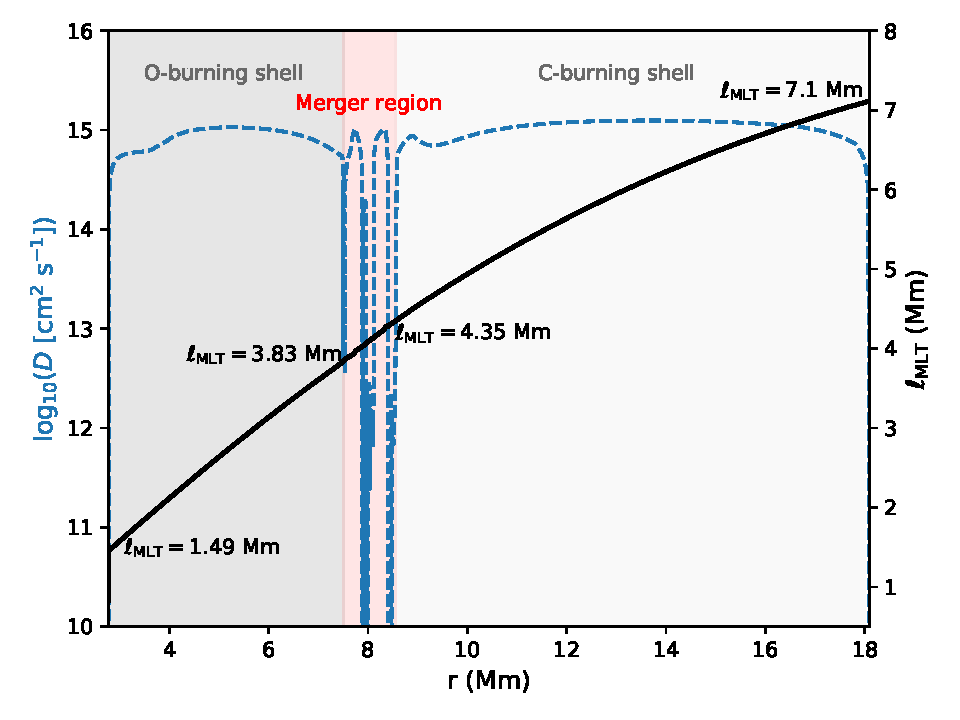
\includegraphics[width=\textwidth]{chapters/1/figures/Oshell_ell_MLT.pdf}
\caption{O-burning shell of the $15 M_\odot$ $Z=0.02$ model from \cite{ritterNuGridStellarData2018} at model number 9200 right before the merger with C-shell is fully realized. The O-shell is from $2.79~\mathrm{Mm}$ to $7.49~\mathrm{Mm}$, the merger region is from $7.49~\mathrm{Mm}$ to $8.56~\mathrm{Mm}$, and the C-burning shell is from $8.56~\mathrm{Mm}$ to $18~\mathrm{Mm}$.
\label{fig:Oshell_ell_MLT}}
\end{figure}

As recognized by \cite{bazanConvectionNucleosynthesisCore1994}, the O-burning shell cannot adequately be described by MLT.
For example, Figure \ref{fig:Oshell_ell_MLT} shows the $15 M_\odot$ $Z=0.02$ model from \cite{ritterNuGridStellarData2018} as it is merging.
The O-burning shell has a size of $4.7~\mathrm{Mm}$, merging region $1.07~\mathrm{Mm}$, and C-burning shell $9.44~\mathrm{Mm}$.
At best, the regions can resolve $3.2$, $0.3$, and $2.2$ fluid elements respectively.
Clearly, these regions are not well resolved by MLT -- especially the merger region.
INSERT THIS PARAGRAPH HERE

\subsection{3-D Simulations of Convective O-Shell Burning and C-Shell Entrainment}

Multidimensional hydrodynamic simulations have been done of O-shell burning and C-shell entrainment in massive stars.
\cite{bazanConvectionNucleosynthesisCore1994} performed a 2-D simulation of O-burning where they show that the convective motions and temperature are non-radially, spherically asymmetric and mix through radiative layers by a penetrative convection rather than a simple overshoot.

\cite{meakinActiveCarbonOxygen2006} performed a 2-D simulation of both the O- and C-burning shells with a limited nuclear network and compared to a 3-D simulation of just the O-shell.
They found that the non-convective region between the two shells had comparable velocities to the convective shells and that the convective shells have large, round vortices and asymmetric density perturbations.
Additionally, they found that the convective motions excited waves in the radiative layer that allowed for C-shell entrainment into the O-shell at $\sim10^{-4} M_\odot s^{-1}$.
Because of this entrainment, they found there would be sudden O-flames burning in the O-shell that would turn on and off.
However, they note that their 3-D O-shell simulation show plumes rather than vortices to describe the flow and caution against using 2-D simulations to describe the convective motions in this scenario. 

\cite{meakinTurbulentConvectionStellar2007} also find this mixing difference between 2 and 3-D simulation of O-shells, and they also find that the 3-D radial velocity decreases gradually at the top of the shell and sharply at the bottom, which cannot be explained by a constant $\alpha_{\mathrm{MLT}}$.
This is explained by the distance to the convective boundary acting as an upper limit to the mixing length, as fluid elements cannot travel a full mixing length if the remaining space they have is less than it.
They also find turbulent entrainment of material from the stable layer above the O-shell. 

\cite{jonesIdealizedHydrodynamicSimulations2017} in their 3-D simulation of O-shell burning that the 3-D radial velocity profile exhibits the same gradual decrease at the upper boundary and find an entrainment from the stable layer of $1.33\times10^{-6}M_\odot s^{-1}$.
\begin{figure}[!htbp]
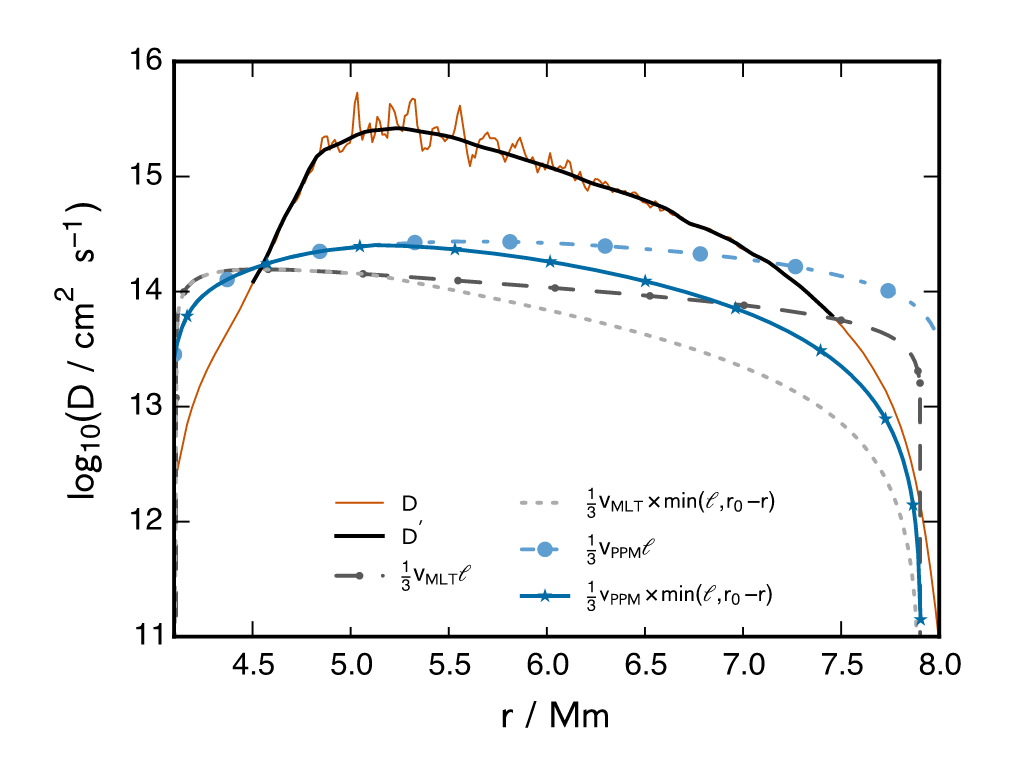
\includegraphics[width=\textwidth]{chapters/1/figures/Jones+17_Fig21.png}
\caption{Taken from \cite{jonesIdealizedHydrodynamicSimulations2017}: Time-averaged radial diffusion coefficient profile calculated from the spherically averaged abundance profiles by the method described in Section 3.5 (brown solid line; black solid line is a fit to the noisy region). The convective velocities computing using MLT agree with the spherically averaged 3D velocities to within about a factor of 2 inside the convection zone but are too large in the vicinity of the CB, resulting in an overestimation of the diffusion coefficient there. Limiting the mixing length to the distance from the CB reproduces the fall-off of the diffusion coefficient inside the convection zone approaching the boundary which is seen in the spherically averaged 3D simulation results.
\label{fig:Jones17_Fig21}}
\end{figure}
As they show in Figure \ref{fig:Jones17_Fig21}, the diffusion coefficient from MLT does not match the shape of what is estimated in 3-D as well underestimating the velocities.
However, they provide a recommendation for 1-D modelling to better match the 3-D diffusion profile shape:
\begin{equation}
    D_{\mathrm{RCMD}} = v_{\mathrm{MLT}}\times\min(\alpha H_\mathrm{P},|r-r_{\mathrm{SC}}|)
\end{equation}
where $\alpha H_\mathrm{{P}}=\ell$ is the mixing length, $r$ is the radius in the convective region, and $r_{\mathrm{SC}}$ is the distance to the convective boundary.
This is rooted in the same insight by \cite{meakinTurbulentConvectionStellar2007} that fluid elements may be too close to the convective boundary to move a full mixing length.
In addition to this, they apply the same insight of distance to convective boundary to convective overshooting and find good agreement with the spherically average 3-D $D$.

\cite{arnett3DSimulationsMLT2019} -- I honestly don't understand this one yet

\cite{yadavLargescaleMixingViolent2020a} in their 3-D simulation of an O-Ne shell merger where they find 3-D has much faster convective velocities than predicted in 1-D, and as the Ne-shell merges strong plumes carry the material to the bottom of the O-shell where burn in a convective-reactive environment.
The asymmetric plume distribution leads to local hotspots of burning causing as difference in the Si, O, and Ne mass fractions when compared to 1-D.

\cite{andrassy3DHydrodynamicSimulations2020} performed 3-D simulation of C-ingestion into a convective O-shell and found a range of possible ingestion rates from $9.5\times10^{-8} M_\odot s^{-1}$ to $1.18\times10^{-8} M_\odot s^{-4}$ and $v_{\mathrm{rms}}$ from $38 \mathrm{km~s^{-1}}$ to $181 \mathrm{km~s^{-1}}$ depending on the luminosity of $^{12}\mathrm{C}+^{12}\mathrm{C}$, $^{16}\mathrm{O}+^{16}\mathrm{O}$, and $^{12}\mathrm{C}+^{16}\mathrm{O}$.
In their simulations they find large scale asymmetries in the luminosity and density during entrainment.
The radial velocity profile they find exhibits a gradual decline at the top of the O-shell, but also a less steep decline at the bottom of the shell.
In addition to this, they boost the energy of C-burning and find large scale asymmetric oscillations like the Global Oscillation of Shell H-ingestion (GOSH) as found in \cite{herwigGLOBALNONSPHERICALOSCILLATIONS2014}.
GOSHs can lead to increased entrainment of material, but also quench convective motions.

\cite{rizzutiShellMergersLate2024a} performed a 3-D hydrodynamic simulation of an O-C shell merger with a limited nuclear network and find significant differences from their 1-D model.
In the 1-D model, the top convective boundary of the O-shell grows until it merges with the Ne/C-shell above it, but in the 3-D simulation the bottom of the C-shell grows until it merges with the Ne and O-shells under it.
Like \cite{jonesIdealizedHydrodynamicSimulations2017}, they find that 1-D convective velocities are a few factors lower than the 3-D simulation.
Because of the differences in 1-D and 3-D they find that there are significant differences in the mass fraction of species like $^{20}\mathrm{Ne}$, $^{24}\mathrm{Mg}$, and $^{28}\mathrm{Si}$.

\subsection{1-D Implementation of 3-D Hydrodynamics}\label{sec:intro_1dimplementof3d}

Despite the insufficiencies of 1-D stellar evolution, 3-D hydrodynamic codes are unable to calculate the nucleosynthesis for complex processes such as the $\gamma$-process where thousands of isotopes can be involved.
Nucleosynthetic yields have to be calculated then in 1-D, but the insufficiencies of 1-D can be mitigated by adopting the results of 3-D hydrodynamics and testing a variety of mixing scenarios.
Specific to O-shell burning in O-C shell mergers, the following are possible to investigate in 1-D to explore the impact on nucleosynthesis.

\begin{itemize}
\item The shape of the radially averaged 3-D diffusion coefficient profile exhibits a  downturn at the boundaries of the O-shell that is not seen in 1-D \citep{meakinTurbulentConvectionStellar2007, jonesIdealizedHydrodynamicSimulations2017}.
\item Convective velocities are higher in 3-D hydrodynamic simulations than predicted by mixing length theory \citep{jonesIdealizedHydrodynamicSimulations2017, rizzutiShellMergersLate2024a}.
\item The entrainment rate of C-shell material into the O-shell could be anywhere from $10^{-8}M_\odot \mathrm{s^{-1}}$ to $10^{-4}M_\odot \mathrm{s^{-1}}$ \citep{andrassy3DHydrodynamicSimulations2020}.
\item Asymmetric non-radial instabilities are present due to energy feedback which could lead to convective quenching \citep{andrassy3DHydrodynamicSimulations2020}. 
\end{itemize}

To address the shape a gradual downturn to $D_{\mathrm{conv}}$ Equation \ref{eq:d_mlt} from \cite{jonesIdealizedHydrodynamicSimulations2017} is adopted, but at the bottom of the O-shell instead of the top.
This is done because we are simulating the nucleosynthesis during an O-C shell merger, and so the upper convective boundary is already connected to the C-shell above.
To address lower convective velocities in 1-D, a series of boost factors can be applied to $D$.
To address the variability of C-shell entrainment, a variety of entrainment rates can be adopted in a 1-D post-processed model.
Finally, to address energy feedback such as the GOSH-like events seen in \cite{andrassy3DHydrodynamicSimulations2020}, a simple dip in the convective profile can be adopted:
\begin{equation}
D_{\mathrm{dip}}=D_{\mathrm{MLT}}-(D_{\mathrm{MLT}}-c)\times\exp\Biggl[-\frac{(r-a)^2}{w^2}\Biggr]
\end{equation}
where $c$ is the depth of the dip, $a$ is the location of the dip, and $w$ is width of the dip.
Using the results of 3-D hydrodynamic simulations, we can explore the possible impact on nucleosynthesis from macrophysics.